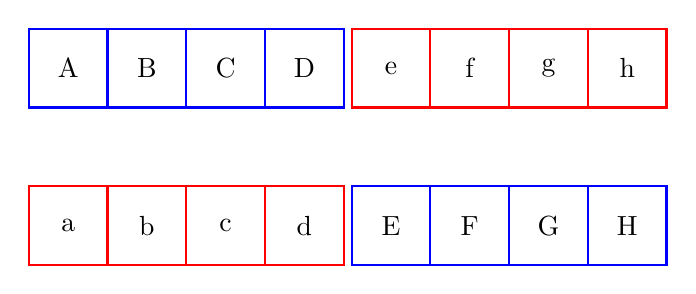
\begin{tikzpicture}
	
	%nodes in the red genome have names of the form r1, r2 ...
	%nodes in the blue genome have names of the form b1,br2 ...

	%for orientation: find the red ball
	%\draw [fill=red] (rb) circle (0.2);


	\def\xskip{0.1}
	\def\yskip{-2}
		 

	%blue, upper left
	\foreach \genomepoint/\position in {A/1, B/2,  C/3,  D/4}
   {
		\draw [blue, thick] (\position -0.5, 0 -0.5 ) rectangle (\position + 0.5,0.5) ;
		\node (b\genomepoint) at (\position,0) {\genomepoint};
   }
	
	%red, lower left
\foreach \genomepoint/\position in {a/1,  b/2,  c/3,  d/4}
   {
		\draw [red, thick] (\position -0.5, \yskip -0.5 ) rectangle (\position + 0.5, \yskip +0.5) ;
		\node (r\genomepoint) at (\position, \yskip) {\genomepoint};
   }

	%red. upper right
\foreach \genomepoint/\position in {e/5,  f/6,  g/7,  h/8}
   {
		\draw [red, thick] (\xskip + \position -0.5,  -0.5 ) rectangle (\xskip + \position + 0.5, 0 +0.5) ;
		\node (r\genomepoint) at (\xskip + \position, 0) {\genomepoint};
   }


	%blue. lower right
\foreach \genomepoint/\position in {E/5,  F/6,  G/7,  H/8}
   {
		\draw [blue, thick] (\xskip + \position -0.5, \yskip -0.5 ) rectangle (\xskip + \position + 0.5, \yskip +0.5) ;
		\node (b\genomepoint) at (\xskip + \position, \yskip) {\genomepoint};
   }


\end{tikzpicture}